Lo studio del moto di una particella soggette a potenziali di forma arbitraria risulta molto complicato, in particolar modo nel contesto della relatività nella quale le equazioni di Eulero Lagrange danno origine ad equazioni differenziali più complesse delle loro analoghe classiche, per questo motivo si limiterà lo studio al caso di campi costanti. 
\subsection{Campo elettrico costante}
Si consideri un campo solamente elettrico, ossia in cui $\vec B=0$, costante nel tempo ed uniforme, questo campo è orientato in una direzione spaziale determinata. Il sistema quindi perde la sua proprietà di isotropia spaziale ma lo spazio permane isotropo, per questo motivo è possibile orientare a piacere gli assi del sistema di riferimento così che: $\vec E$ risulti parallelo all'asse $x$ e l'asse $y$ parallelo alla velocità iniziale della carica e quindi il moto avvenga nel piano $xy$. Dalla \eqref{PotenzialiCostanti} si ha che il potenziale scalare può quindi essere espresso come $\varphi=|\vec E|x$, con $|\vec E|$ intensità del campo.
Utilizzando questo potenziale le equazioni di Eulero Lagrange risultano in:
\begin{equation*}
    \dot p_x=q|\vec E|,\quad\dot p_y=0,\quad\dot p_z=0 \quad \Rightarrow \quad p_x=q|\vec E|t,\quad p_y=p_0,\quad p_z=0.
\end{equation*}
Facendo uso della relazione energia-impulso \eqref{relazioneEnergiaImpulso} si ottiene l'energia di corpo libero della particella ad un determinato istante:
\begin{equation*}
    E_{Lib}=\sqrt{m^2c^4+c^2p_0^2+(cq|\vec E|t)^2}=mc^2\gamma.
\end{equation*}
Questa espressione dell'energia consente tramite la \eqref{velPE} di ottenere un'espressione istante per istante della velocità del corpo:
\begin{equation*}
    v_x=\frac{p_xc^2}{E_{Lib}}=\frac{c^2q|\vec E|t}{\sqrt{m^2c^4+c^2p_0^2+(cq|\vec E|t)^2}},\quad v_y=\frac{p_yc^2}{E_{Lib}}=\frac{c^2p_0}{\sqrt{m^2c^4+c^2p_0^2+(cq|\vec E|t)^2}},\quad v_z=0.
\end{equation*}
Integrando rispetto al tempo queste tre espressioni si ottengono le equazioni del moto a meno di costanti additive:
\begin{flalign}
    x(t)&=\int_{0}^{t}\frac{c^2q|\vec E|t}{\sqrt{m^2c^4+c^2p_0^2+(cq|\vec E|t)^2}}\ dt=\frac{\sqrt{m^2c^4+c^2p_0^2+(cq|\vec E|t)^2}}{q|\vec E|}+C_x,\label{MotoEConstX}\\
    y(t)&=\int_{0}^{t}\frac{c^2p_0}{\sqrt{m^2c^4+c^2p_0^2+(cq|\vec E|t)^2}}\ dt=\frac{p_0c}{q|\vec E|}\text{arsinh}\bigg(\frac{cq|\vec E|t}{\sqrt{m^2c^4+c^2p_0^2}}\bigg)+C_y,\label{MotoEConstY}\\
    z(t)&=C_z.
\end{flalign}
Posti $x(0)=y(0)=z(0)=0$, se si esprime nell'equazione del moto lungo l'asse $y$ \eqref{MotoEConstY} il tempo rispetto ad $y$ e lo si sostituisce nell'equazione del moto nella direzione dell'asse $x$ \eqref{MotoEConstX} si ottiene la traiettoria che compie la particella nel piano $xy$:
\begin{equation}
    x(y)=\frac{\sqrt{m^2c^4+c^2p_0^2}}{q|\vec E|}\bigg[\cosh\bigg(\frac{q|\vec E|y}{c\sqrt{m^2c^4+c^2p_0^2}}\bigg)-1\bigg].
\end{equation}
\begin{figure}[H]
    \centering
    \begin{subfigure}{.3\textwidth}
        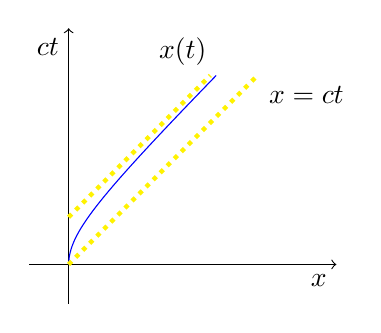
\begin{tikzpicture}
           \draw[->] (0,-.5)--(0,3)node[anchor=north east]{$ct$};
           \draw[->] (-.5,0)--(3.4,0)node[anchor=north east]{$x$};
           \draw[scale=.6, domain=0:4, smooth, variable=\x, blue] plot ( {sqrt(1+\x*\x)-1},{\x}) node[anchor= south east, color=black ]{$x(t)$};
           \draw[scale=.6, domain=0:4, smooth, variable=\x, yellow,ultra thick,dotted] plot ( {\x},{\x}) node[anchor= north west, color=black ]{$x=ct$};
           \draw[scale=.6, domain=1:4, smooth, variable=\x, yellow,dotted, ultra thick] plot ( {\x-1},{\x});
       \end{tikzpicture}   
       \end{subfigure}
       \begin{subfigure}{.3\textwidth}
        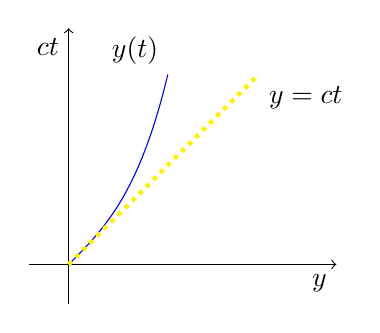
\begin{tikzpicture}
           \draw[->] (0,-.5)--(0,3)node[anchor=north east]{$ct$};
           \draw[->] (-.5,0)--(3.4,0)node[anchor=north east]{$y$};
           \draw[scale=.6, domain=0:2.1, smooth, variable=\x, blue] plot ( {\x},{sinh(\x)}) node[anchor= south east, color=black ]{$y(t)$};
           \draw[scale=.6, domain=0:4, smooth, variable=\x, yellow,ultra thick,dotted] plot ( {\x},{\x}) node[anchor= north west, color=black ]{$y=ct$};
       \end{tikzpicture}   
       \end{subfigure}
    \begin{subfigure}{.3\textwidth}
     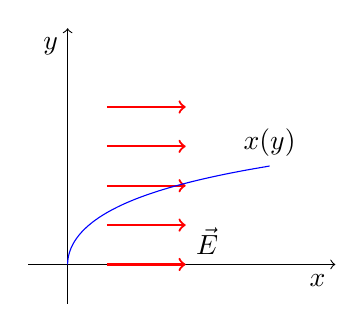
\begin{tikzpicture}
        \draw[thick,red,->] (.5,0.5)--(1.5,.5);
        \draw[thick,red,->] (.5,1)--(1.5,1);
        \draw[thick,red,->] (.5,1.5)--(1.5,1.5);
        \draw[thick,red,->] (.5,2)--(1.5,2);
        \draw[->] (0,-.5)--(0,3)node[anchor=north east]{$y$};
        \draw[->] (-.5,0)--(3.4,0)node[anchor=north east]{$x$};
        \draw[thick,red,->] (.5,0)--(1.5,0)node[anchor=south west, black]{$\vec{E}$};
        \draw[scale=.5, domain=0:2.5, smooth, variable=\x, blue] plot ( {cosh(\x)-1},{\x}) node[anchor= south, color=black ]{$x(y)$};
    \end{tikzpicture}   
    \end{subfigure}
    \caption{Rappresentazione grafica delle equazioni del moto ottenute.}
    \label{fig:motoECost}
\end{figure}
 In figura \ref{fig:motoECost} è possibile apprezzare che per $t\rightarrow \infty$ si ha $v_x\rightarrow c$ e $v_y\rightarrow 0$: infatti anche se la forza di Lorentz è diretta solo nella direzione dell'asse $x$ la particella decelera anche nella direzione dell'asse $y$ affinché il moto  sia sempre racchiuso nel cono di luce.

\subsection{Campo magnetico costante}
Se si considera solamente un campo magnetico uniforme, come si è fatto per il campo elettrico costante, è possibile orientare il sistema di riferimento in maniera tale da avere tale campo diretto lungo l'asse $z$. In questo modo il potenziale vettore dalla relazione \eqref{PotenzialiCostanti} risulta $\vec A=\frac{|\vec B|}{2}(-y,x,0)$, dove $|\vec B|$ è il modulo del campo magnetico.\\ Si osservi che, essendo la lagrangiana di questo sistema indipendente dal tempo, l'energia del sistema si conserva e dalla \eqref{energiaImpulsoIntEM} questa, in assenza di campi elettrici, è $E=mc^2\gamma$.\\Usando le equazioni di Eulero Lagrange e la relazione \eqref{velPE} si ottiene:
\begin{equation*}
    \dot{p}_x=qv_y |\vec B|=\frac{d}{dt}\bigg(\frac{v_xE}{c^2}\bigg),\quad \dot{p}_y=-qv_x|\vec B|=\frac{d}{dt}\bigg(\frac{v_yE}{c^2}\bigg)\quad\Rightarrow\quad \dot v_x=v_y\frac{|\vec B|q}{m\gamma},\quad\dot v_y=-v_x\frac{|\vec B|q}{m\gamma}.
\end{equation*}
Per risolvere questo sistema di equazioni differenziali si osservi che se definisce la quantità $v_x+iv_y$, dove $i^2=-1$, è possibile ricondursi un'equazione differenziale a variabili separabili:
\begin{equation*}
    \frac{d}{dt}(v_x+iv_y)=-i\frac{|\vec B|q}{m\gamma}(v_x+iv_y)\quad\Rightarrow\quad v_x+iv_y=v_0e^{-i\frac{|\vec B|q}{m\gamma}t+i\alpha}
\end{equation*}
dove $\alpha=\arctan\frac{v_y(0)}{v_x(0)}$ e $v_0^2=v_x^2(t)+v_y^2(t)$ sono due costanti da determinare.\\
Separando la parte immaginaria e la parte reale di quanto ottenuto e integrando nuovamente si ottengono le equazioni del moto:
\begin{flalign}
    v_x(t)&=v_0\cos\bigg(\frac{|\vec B|q}{m\gamma}t+\alpha\bigg)\quad&\Rightarrow\quad &x(t)=x_0+\frac{v_0m\gamma}{|\vec B|q}\sin\bigg(\frac{|\vec B|q}{m\gamma}t+\alpha\bigg)&&\\
    v_y(t)&=-v_0\sin\bigg(\frac{|\vec B|q}{m\gamma}t+\alpha\bigg)\quad&\Rightarrow\quad &y(t)=y_0+\frac{v_0m\gamma}{|\vec B|q}\cos\bigg(\frac{|\vec B|q}{m\gamma}t+\alpha\bigg)&&\\
    v_z(t)&=v_z \quad &\Rightarrow\quad &z(t)=z_0+v_zt.&&
\end{flalign}
Proiettando il moto nel piano $xy$ si ottiene una circonferenza centrata in $(x_0,y_0)$ e di raggio $r=\frac{v_0m\gamma}{|\vec B|q}$ che nel complesso da origine ad un'elica nello spazio.
\begin{figure}[H]
    \centering
    \begin{subfigure}{.3\textwidth}
        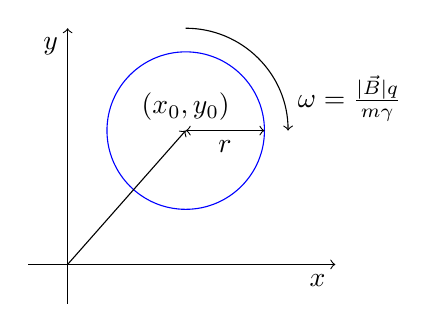
\begin{tikzpicture}
           \draw[->] (0,-.5)--(0,3)node[anchor=north east]{$y$};
           \draw[->] (-.5,0)--(3.4,0)node[anchor=north east]{$x$};
           \draw[color=blue,] (1.5,1.7) circle (1);
           \draw[->] (0,0) -- (1.5,1.7) node[anchor=south]{$(x_0,y_0$)};
           \draw[<->] (1.5,1.7) --node[anchor=north]{$r$} (2.5,1.7);
           \draw[<-] (2.8,1.7)node[anchor=south west]{$\omega=\frac{|\vec B|q}{m\gamma}$} arc(0:90:1.3) ;
       \end{tikzpicture}
    \end{subfigure}   
    \begin{subfigure}{.3\textwidth}
     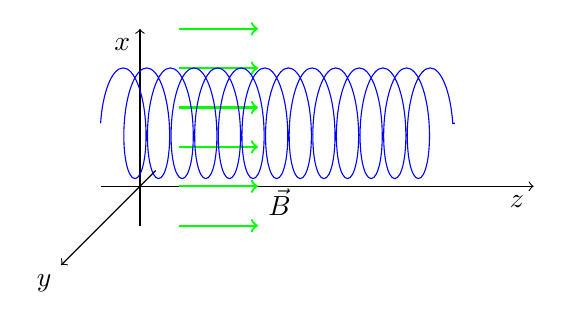
\begin{tikzpicture}
        \draw[thick,green,->] (.5,0.5)--(1.5,.5);
        \draw[thick,green,->] (.5,1)--(1.5,1);
        \draw[thick,green,->] (.5,1.5)--(1.5,1.5);
        \draw[thick,green,->] (.5,2)--(1.5,2);
        \draw[thick,green,->] (.5,-.5)--(1.5,-.5)node[anchor=south west, black]{$\vec{B}$};
        \draw[->] (0,-.5)--(0,2)node[anchor=north east]{$x$};
        \draw[->] (0.2,.2)--(-1,-1)node[anchor=north east]{$y$};
        \draw[->] (-.5,0)--(5,0)node[anchor=north east]{$z$};
        \draw[thick,green,->] (.5,0)--(1.5,0);
        \draw[decoration={aspect=0.3, segment length=3mm, amplitude=20,coil},decorate,color=blue] (-0.5,.8) -- (4,.8); 
    \end{tikzpicture}   
    \end{subfigure}
    \caption{Rappresentazione grafica delle equazioni del moto ottenute.}
    \label{fig:motoBCost}
\end{figure}
 Il risultato ottenuto è simile a quanto è predetto dalla meccanica classica, differisce da questa per il valore esatto della frequenza di rotazione e del raggio che dipendo da $\gamma$ e si riconducono alle loro forme newtoniane nel limite classico per cui $\gamma \approx 1$.